\section{Measured and analytical efficiency}
\label{sec:supp_efficiency}
We measure LLaVA-3D-7B efficiency under the default GeoGate schedule, distinguishing application time from generation-core timing. Application time decreases by 0.8--1.4\%, whereas generation-core timing and analytical LM estimates cover narrower computational scopes. We report both timing boundaries, followed by tensor-batch throughput and analytical LM cost. \Cref{fig:supp_original_teaser} summarizes these distinct measurements, which do not establish quality superiority at matched measured cost.

\begin{figure*}[t]
\centering
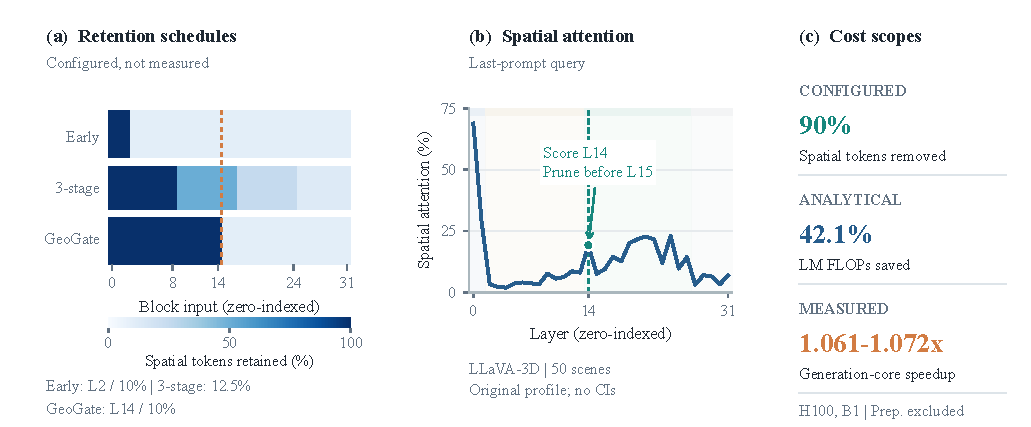
\includegraphics[width=\textwidth]{fig_teaser.pdf}
\caption{Tested schedule and distinct evidence scopes. Retention schedules, attention profiles, analytical LM cost, and measured generation speed describe different quantities. Their juxtaposition establishes neither matched-cost quality dominance nor independent quality preservation.}
\label{fig:supp_original_teaser}
\end{figure*}

\subsection{Generation and application time at batch size one}
Each batch-size-one session loads both conditions once and alternates their order across questions. It uses ten warm-up questions and synchronizes CUDA around generation, with inputs GPU resident when timing begins. \Cref{tab:supp_b1} reports the three full-set sessions separately.

\begin{table}[t]
\centering
\caption{Paired generation-core timing on one H100, batch size one. Times in milliseconds are condition-wise medians. The ratio is the median of paired per-question GeoGate/native times, not the quotient of the two medians.}
\label{tab:supp_b1}
\begin{tabular}{lccc}
\toprule
Session & Native & GeoGate & Paired ratio \\
\midrule
1 & 160.20 & 150.60 & 0.9429 \\
2 & 159.98 & 150.41 & 0.9411 \\
3 & 144.97 & 135.13 & 0.9324 \\
\bottomrule
\end{tabular}
\end{table}

Generation-core ratios correspond to reciprocal speedups of $1.061\times$, $1.063\times$, and $1.072\times$. Broader application-time ratios are 0.9921, 0.9910, and 0.9855, representing reductions of 0.8--1.4\%. This broader boundary includes preprocessing, transfer, generation, and decoding. Median allocation increments decrease from 1,613 to 1,052 MiB, excluding parameters and inputs that are already resident.

\subsection{Same-scene tensor batches}
The B2/B4 runs (\Cref{tab:supp_batch}) use tensor batches of questions from the same scene and include remainder-padding time in the useful-throughput denominator. Three fresh processes each evaluate all 4,675 questions. Validation covers 18,972 raw rows, 3,569 multimodal preparations, and 7,138 model calls; all checks pass in every process.

\begin{table*}[t]
\centering
\caption{Controlled same-scene tensor-batch throughput on one H100. Each useful q/s value is the real-question count divided by summed batch generation time, including padding time. The throughput ratio is native total time divided by GeoGate total time; intervals target this ratio.}
\label{tab:supp_batch}
\begin{tabular}{cccccc}
\toprule
Batch & Session & Native useful q/s & GeoGate useful q/s & Total-time ratio & Scene 95\% CI \\
\midrule
2 & 1 & 5.548 & 6.189 & 1.115 & [1.101, 1.130] \\
2 & 2 & 5.456 & 6.056 & 1.110 & [1.094, 1.125] \\
2 & 3 & 5.469 & 6.063 & 1.109 & [1.094, 1.123] \\
4 & 1 & 6.559 & 7.691 & 1.172 & [1.155, 1.189] \\
4 & 2 & 6.679 & 7.893 & 1.182 & [1.165, 1.198] \\
4 & 3 & 6.589 & 7.755 & 1.177 & [1.160, 1.193] \\
\bottomrule
\end{tabular}
\end{table*}

All 4,675 EOS-trimmed outputs reproduce exactly across processes within each batch-size/condition cell. GeoGate does not generate shorter answers: mean lengths increase by 0.021 tokens at B2 and 0.047 at B4, while medians and P95 values are identical. These results measure GPU-resident generation with homogeneous same-scene batches, rather than end-to-end serving.

\subsection{Mixed-scene heterogeneous batches}
The v18c follow-up (\Cref{tab:supp_hetero_batch}) tests heterogeneous batching while keeping the frozen model, prompts, seed, B4 schedule size, and generation-core timing boundary. Three fresh processes each evaluate all 4,675 questions. Among 1,169 batches, 1,168 contain at least two scenes and at least two visual-token counts. The predeclared terminal remainder contains three real questions and one padding slot.

Each batch's elapsed time, including padding, is divided equally among its real questions. Summing these allocations over the full set counts each batch time exactly once. The total-time ratio therefore compares native and GeoGate generation-core time under the recorded schedule. The displayed rates instead summarize median allocated time per question.

\begin{table*}[t]
\centering
\caption{Mixed-scene heterogeneous B4 generation on one H100. The rate columns (q/s) are reciprocals of condition-wise median allocated time per real question. The total-time ratio instead divides summed native allocated times by summed GeoGate times. Frozen scene intervals refer to this ratio under the allocation-based procedure; coverage for shared batch timing and between-session variation remains unvalidated. Dividing the displayed rate columns does not recover the ratio.}
\label{tab:supp_hetero_batch}
\begin{tabular}{cccccc}
\toprule
Session & Native rate & GeoGate rate & Total-time ratio & Scene 95\% CI & Mean length delta \\
\midrule
1 & 5.557 & 6.065 & 1.088 & [1.082, 1.094] & +0.0077 \\
2 & 5.532 & 6.053 & 1.091 & [1.084, 1.098] & +0.0015 \\
3 & 5.651 & 6.181 & 1.091 & [1.084, 1.098] & +0.0077 \\
\bottomrule
\end{tabular}
\end{table*}

The frozen bootstrap samples scenes jointly for native and GeoGate, preserving question pairing and each scene's question group. However, the 1,168 mixed batches share measured times across scenes. Scene resampling can give different multiplicities to portions of the same batch time, so it does not preserve batch-level timing dependence. We retain these intervals as scene-reweighting summaries conditional on the recorded schedule and allocation. Their coverage for execution-time variation has not been established; the per-session intervals also do not estimate between-process uncertainty. This limitation establishes neither the direction nor the magnitude of any interval-coverage error.

All three sessions meet the throughput criterion under the recorded decision procedure. GeoGate has identical median and P95 answer lengths, and its mean length is not shorter. However, 73 of 18,700 question-condition pairs differ across processes despite matching input-tensor hashes for all 9,352 slots. Exact output reproduction across processes is therefore not established.

A bounded repeat diagnostic examines eight batches from the three scenes exceeding the 2,560-token preparation cap. Each condition order is repeated three times, comparing EOS-trimmed token sequences. Input-tensor hashes and GeoGate pruning traces match, but 15 of 32 condition-order groups produce multiple sequences (6 baseline and 9 GeoGate groups). This demonstrates non-bitwise generation within the tested runner, beyond cross-process or condition-order differences. Backend isolation repeats seven of these batches: native SDPA with GPU scatter yields 13/28 stable same-order groups, math SDPA 13/28, eager attention 12/28, and ordered CPU-reference voxel scatter 13/28. Inputs and pruning traces match throughout. The instability is therefore not isolated to these attention or scatter kernels.

Post-hoc exclusion of the 58 questions with any cross-process mismatch leaves 4,617 questions per session. Throughput ratios remain $1.088$--$1.092$, with frozen scene lower bounds above $1.082$. This calculation retains parts of some batch-time allocations; it does not measure a rerun of the smaller workload. It therefore shares the interval-dependence limitation above. The recorded throughput rule uses per-batch timing and does not require bitwise output identity. These ratios characterize generation-core throughput in the evaluated sessions, without establishing token determinism, quality equivalence, or end-to-end serving speedup.

\subsection{Analytical LM cost and decode length}
The analytical LM proxy uses hidden width $d=4096$, feed-forward width $I=11008$, and $L=32$ decoder blocks. Per-layer prefill cost is $f(s)=4sd^2+2s^2d+3sdI$; one-step decode cost is $h(k)=4d^2+2kd+3dI$. GeoGate prefills 15 full-length and 17 reduced-length blocks. After all-layer prompt-cache compaction, the decode proxy uses $k=T_{\text{kept}}=370$ at every block, versus $T=1717$ for native. Cache lengths remain fixed throughout the assumed decode steps, excluding generated-token growth. The KV ratio $370/1717$ therefore estimates prompt storage at decode initialization, not final answer-cache size. Vision, token selection, cache indexing, and total GPU allocation lie outside this analytical model.

The reported analytical ratio assumes eight decode steps. \Cref{tab:supp_cost_sensitivity} evaluates the same equations for one through 32 steps. The machine-readable results also include mean generation lengths from the three frozen timing sessions. This sensitivity analysis concerns analytical LM cost, not measured latency or full-model FLOPs.

\begin{table}[t]
\centering
\caption{Analytical LM cost ratios across decode lengths.}
\label{tab:supp_cost_sensitivity}
\resizebox{\columnwidth}{!}{%
\begin{tabular}{rccc}
\toprule
Decode steps & GeoGate ratio & GeoGate reduction & FastV minus GeoGate \\
\midrule
1 & 0.5776 & 42.24\% & 1.28 pp \\
2 & 0.5778 & 42.22\% & 1.28 pp \\
4 & 0.5783 & 42.17\% & 1.28 pp \\
8 & 0.5791 & 42.09\% & 1.28 pp \\
16 & 0.5808 & 41.92\% & 1.29 pp \\
32 & 0.5842 & 41.58\% & 1.30 pp \\
\bottomrule
\end{tabular}}
\end{table}

GeoGate's analytical LM cost reduction stays within $41.58$--$42.24\%$ across this range. The FastV L2/R50 total-cost gap remains $1.28$--$1.30$ percentage points. The prefill ratio, $0.5774$, does not depend on the assumed decode budget.
